\documentclass[journal]{IEEEtran}
\usepackage{amsmath, amsfonts, graphicx, balance}
\usepackage{float, subfig}

\graphicspath{ {./images/} } % tells LaTeX that the images are kept in a folder named images under the directory of the main document.

\title{Lab 1: Signal Analysis and Noise Reduction Using MATLAB}
\author{
    \IEEEauthorblockN{Argenis Aquino, Rachel DuBois, Diego Lopez, Jonathan Sumner \\}
    \IEEEauthorblockA{
        Department of Engineering Technology, Rochester Institute of Technology\\
        1 Lomb Memorial Drive, Rochester NY, 14623, United States of America \\
    }
}

\begin{document}
\maketitle

\begin{abstract}
    MATLAB was used to analyze signals and visualize how noise and drift can have an effect on a signals quality. Using the tools provided by MATLAB, such as the plot and variance functions, the signal-to-noise ratio (SNR) was estimated and linear regression was used to determine the drift of a signal. Plots were created in order to compare data gathered such as the original signal to the noisy signal.
\end{abstract}

\section{Introduction}

\IEEEPARstart{M}{ATLAB} is a popular software used in mathematics, science, and engineering for numerical computing and data analysis. Using the tools provided by MATLAB allows for the analysis of signals. This report explores key concepts such as linear drift, linear regression, and signal-to-noise ratio (SNR) estimation.

\section{Results}
Throughout the lab, various plots were created to visualize the data and analyze the signals. The following figures show the original signal, the signal with drift, the signal with no drift, and the noise versus the signal.

\begin{figure}[h] % Fig 1
    \centering
    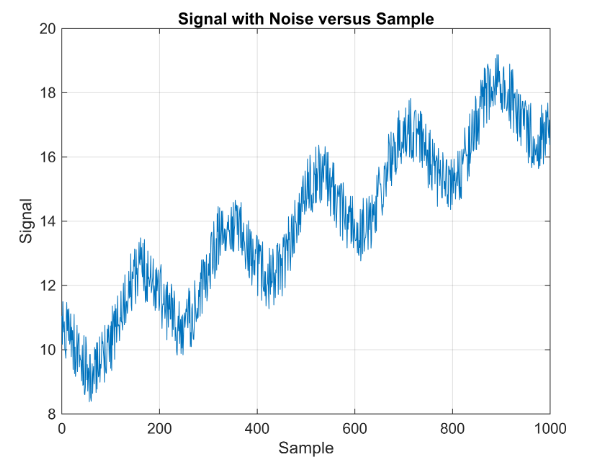
\includegraphics[width=\linewidth]{1.1.png}
    \caption{Original Signal}
    \vspace{1em} % Adds vertical space
    \begin{minipage}{\linewidth}
        \small
        In Figure 1, the original signal is plotted. The signal contains both noise and drift, which can be seen in the graph.
    \end{minipage}
    \label{Part 1: Signal Graph}
\end{figure}

\begin{figure}[ht] % Fig 2
    \centering
    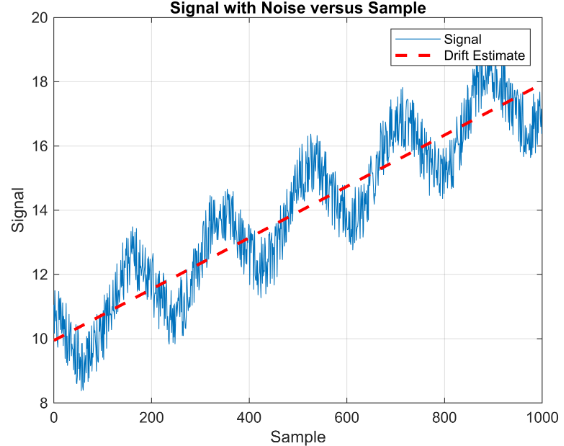
\includegraphics[width=\linewidth]{3.1 plot.png}
    \caption{Graph of the original signal and the fitted line}
    \vspace{1em} % Adds vertical space
    \begin{minipage}{\linewidth}
        \small
        In figure 2, the original signal and the fitted line are displayed. Linear regression was applied to estimate the drift of the signal, with the fitted line helping to visualize the relationship between the sample and the signal.
    \end{minipage}
    \label{Part 3: Fitted Line Graph}
\end{figure}

\begin{figure}[H] % Fig 3
    \centering
    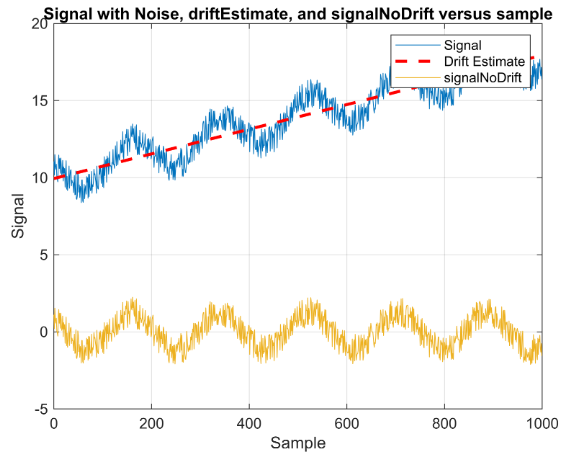
\includegraphics[width=\linewidth]{3.2 plot.png}
    \caption{Graph of the original signal, the signal with drift, and the signal with no drift}
    \vspace{1em} % Adds vertical space
    \begin{minipage}{\linewidth}
        \small
        Figure 3 displays the original signal, the signal with drift, and the signal with no drift. By removing the drift from the signal, a cleaner signal was obtained, as shown in the graph.
    \end{minipage}
    \label{Part 3: No Drift Graph}
\end{figure}

\begin{figure}[ht] % Fig 4
    \centering
    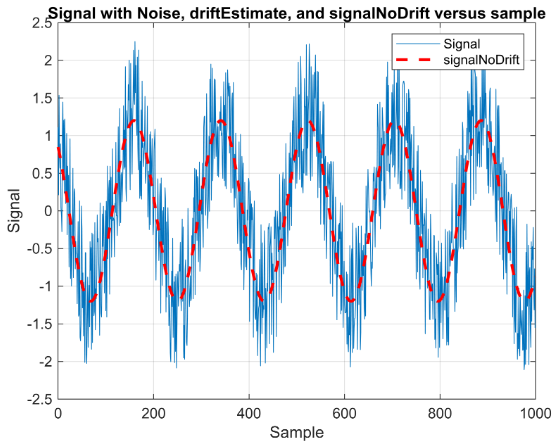
\includegraphics[width=\linewidth]{4.2 plot.png}
    \caption{Graph with the signal with no drift and estimated signal}
    \vspace{1em} % Adds vertical space
    \begin{minipage}{\linewidth}
        \small
        Figure 4 illustrates the signal with no drift and the estimated signal. By estimating the signal and removing the drift, a more accurate representation of the original signal was obtained.
    \end{minipage}
    \label{Part 4: Estimated Signal Graph}
\end{figure}

\begin{figure}[ht] % Fig 5
    \centering
    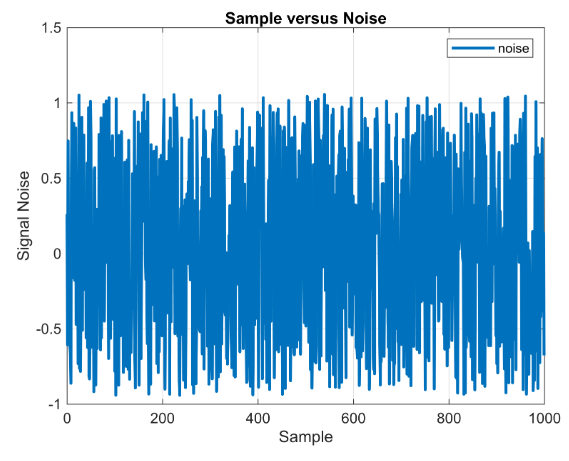
\includegraphics[width=\linewidth]{5.1 plot.png}
    \caption{Graph with the noise versus signal}
    \vspace{1em} % Adds vertical space
    \begin{minipage}{\linewidth}
        \small
        Figure 5 shows the noise versus the signal. By analyzing the relationship between the noise and the signal, the signal-to-noise ratio (SNR) can be estimated.
    \end{minipage}
    \label{Part 5: No Noise Graph}
\end{figure}

\section{Analysis}
In the first part of the lab, a signal was generated and plotted. The plot showed that the signal had both noise and drift.

For the second part of the lab the first step was to use linear regression to estimate the amoun of drift in the signal. Linear regression is a method used to model the relationship between a dependent variable and one or more independent variables. MATLAB has a built-in function called \texttt{polyfit} that can be used to perform linear regression. The \texttt{polyfit} function takes in the x and y values of the data, in this case the sample and signal variables, and the degree of the polynomial to fit the data to. The output of the \texttt{polyfit} function is an array of coefficients of the polynomial that best fits the data. The coefficients are the \texttt{slope} and \texttt{intercept} which are then used to determine the slope of the line which is the drift of the signal.

For the second step of part two we used slope intercept form to determine the drift of the signal. The slope intercept form is given by the equation $y = mx + b$ where $m$ is the slope and $b$ is the y-intercept. The slope and intercept were determined by the coefficients of the polynomial that was fit to the data. The slope was multiplied by the sample and added to the intercept to get the drift estimate.

\vspace{1em} % Adds vertical space
\begin{raggedright}
    \noindent driftEstimate = slope * sample + intercept \hfill (1)
\end{raggedright}

\vspace{1em} % Adds vertical space
In step three the objective was to plot the signal and the fitted line in one graph.

With the drift estimate calculated, it was then possible to caluclate the value of the signal when there was no drift. This was done by subtracting the drift estimate from the signal.

Using this new data a new plot was created to compare the original and the estimated drift signal to the signal with no drift.

Part four of the lab was to estimate the signal-to-noise ratio (SNR) of the signal starting with estamating the signal. The SNR is a measure of the quality of a signal and is calculated by dividing the power of the signal by the power of the noise.

With the given data for the signal frquency, being the period, phase, amplitude, and number of samples, the signal was estimated using the following equation:

\vspace{1em} % Adds vertical space
\begin{raggedright}
    \noindent $\mathrm{y} = A \cdot \sin\left(\frac{2\pi}{T}n + \frac{\Phi}{180}\pi\right) \hfill (2)$

    \vspace{1em} % Adds vertical space
    Given Data: \\
    \noindent $\text{Period } T = 181.8182 \text{ samples}$ \\
    \noindent $\text{Phase } \phi = 135 \text{ degrees}$ \\
    \noindent $\text{Amplitude } A = 1.2$ \\
    \noindent $\text{Number of sample } n = \text{sample}$ \\
    signalEstimate =  A * sin( (2 * pi / T) * n + (Phi / 180) * pi )
    
\end{raggedright}

\vspace{1em} % Adds vertical space

With the estimated signal calculated, the next step was to calculate the noise. The noise was calculated by subtracting the signal with drift removed from the estimated signal.

Next step to get the variance of the original signal, the signal with no drift, the estimated signal, and the noise. To calculate the variance of the signal the MATLAB \texttt{var} function was used.

\vspace{1em} % Adds vertical space
\begin{raggedright}
    \noindent 
    varOrig = var(signal) \\
    varNoDrift = var(signalNoDrift) \\
    varSignal = var(signalEstimate) \\
    varNoise = var(noise) \\
\end{raggedright}

To calculate the SNR the power of the signal was divided by the power of the noise. The SNR was calculated using the following equation:

\vspace{1em} % Adds vertical space
\begin{raggedright}
    \noindent $\mathrm{SNR} = 10 \cdot \log_{10}\left(\frac{\mathrm{Power_{signal}}}{\mathrm{Power_{noise}}}\right) \hfill (3)$
\end{raggedright}

\vspace{1em} % Adds vertical space
Using the variances calculated earlier, the SNR was computed as follows:

\vspace{1em} % Adds vertical space
\begin{raggedright}
    \noindent 
    snrNum = varSignal / varNoise \\
    snrDb = 10*log10(snrNum)
\end{raggedright}

\vspace{1em} % Adds vertical space
The calculated SNR value provided an indication of the quality of the signal, with higher values indicating a better quality signal with less noise.

\section{Conclusion}
In conclusion, MATLAB proved to be an effective tool for analyzing signals and understanding the impact of noise and drift on signal quality. By using linear regression, we were able to estimate the drift in the signal and remove it to obtain a cleaner signal. Additionally, the signal-to-noise ratio (SNR) was calculated to quantify the quality of the signal. The results demonstrated the importance of signal processing techniques in improving the accuracy and reliability of signal analysis.
\end{document}


% \balance
% \end{document}
